% ==================================================================================================
\subsection{Equilibrium health states and rates of transition}
\begin{figure}[H]
  \begingroup\centering
  \begin{subfigure}{0.4\linewidth}
    \includegraphics[width=\linewidth]{{1d-X-health-high-tau=0.1}.pdf}
    \caption{High risk}
    \label{fig:1d-health-high}
  \end{subfigure}
  \begin{subfigure}{0.4\linewidth}
    \includegraphics[width=\linewidth]{{1d-X-health-med-tau=0.1}.pdf}
    \caption{Medium risk}
    \label{fig:1d-health-med}
  \end{subfigure}
  \begin{subfigure}{0.4\linewidth}
    \includegraphics[width=\linewidth]{{1d-X-health-low-tau=0.1}.pdf}
    \caption{Low risk}
    \label{fig:1d-health-low}
  \end{subfigure}
  \begin{subfigure}{0.4\linewidth}
    \includegraphics[width=\linewidth]{{1d-X-health-all-tau=0.1}.pdf}
    \caption{Overall}
    \label{fig:1d-health-all}
  \end{subfigure}
  \\\endgroup
  \caption{Equilibrium health state proportions under different rates of turnover.}
  \label{fig:1d-health}
  \footnotesizeTurnover rate (log scale) is a function of
the duration of time spent in the high risk group $\delta_H$,
where shorter time spent in the high risk group yields faster turnover.
No turnover is indicated by $\delta_H^{-1} = 0.03$,
due to population exit rate $\mu = 0.03$.
\end{figure}
\begin{figure}[H]
  \begingroup\centering
  
\includegraphics[width=\linewidth]{dX-abs-full-legend.pdf}
  \begin{subfigure}{0.33\linewidth}
    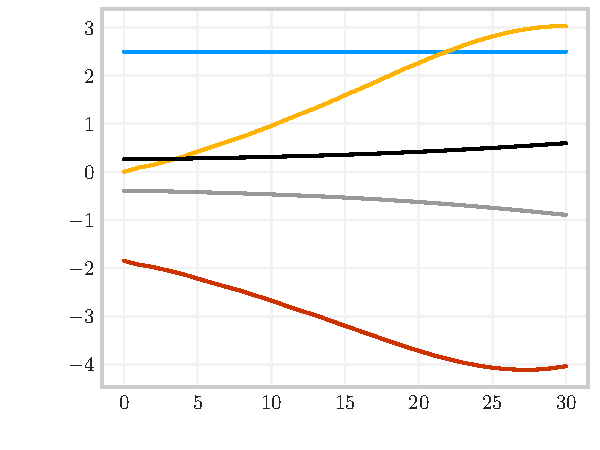
\includegraphics[width=\linewidth]{dX-abs-full-high-S.pdf}
    \caption{High risk susceptible}\label{fig:dX-app-high-S}
  \end{subfigure}%
  \begin{subfigure}{0.33\linewidth}
    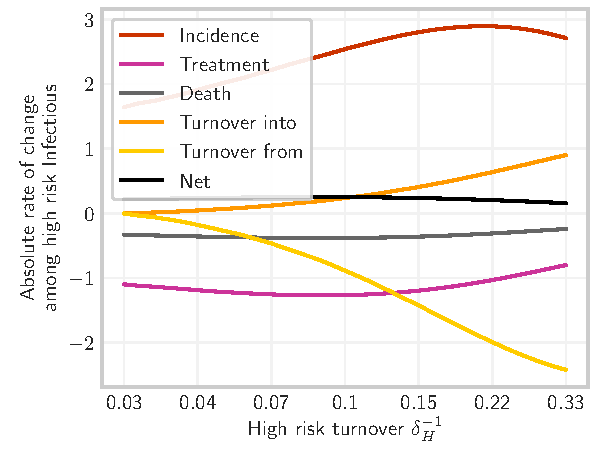
\includegraphics[width=\linewidth]{dX-abs-full-high-I.pdf}
    \caption{High risk infectious}\label{fig:dX-app-high-I}
  \end{subfigure}%
  \begin{subfigure}{0.33\linewidth}
    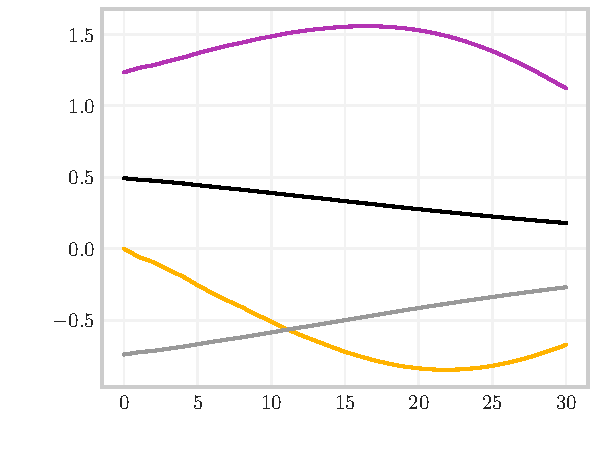
\includegraphics[width=\linewidth]{dX-abs-full-high-T.pdf}
    \caption{High risk treated}\label{fig:dX-app-high-T}
  \end{subfigure}\\
  \begin{subfigure}{0.33\linewidth}
    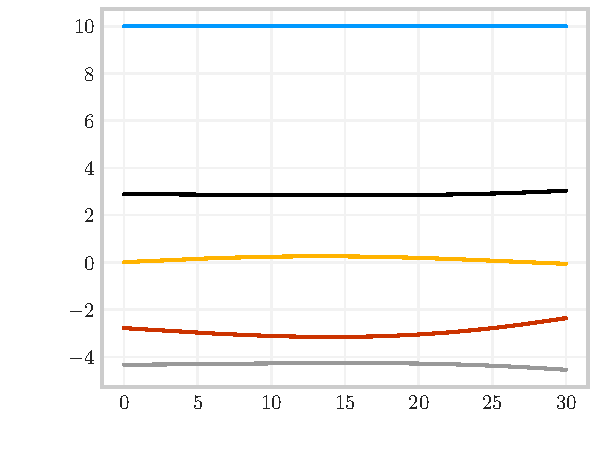
\includegraphics[width=\linewidth]{dX-abs-full-med-S.pdf}
    \caption{Medium risk susceptible}\label{fig:dX-app-med-S}
  \end{subfigure}%
  \begin{subfigure}{0.33\linewidth}
    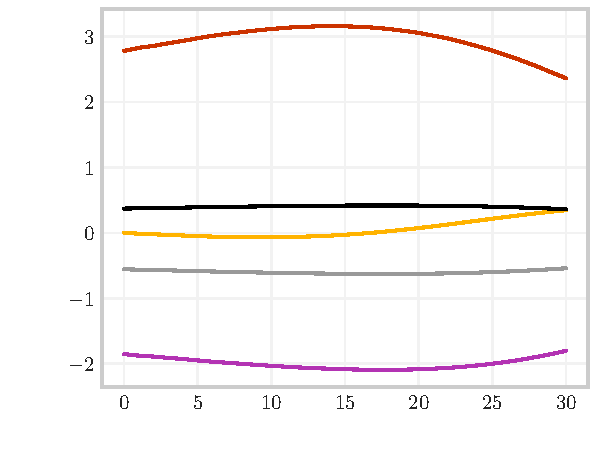
\includegraphics[width=\linewidth]{dX-abs-full-med-I.pdf}
    \caption{Medium risk infectious}\label{fig:dX-app-med-I}
  \end{subfigure}%
  \begin{subfigure}{0.33\linewidth}
    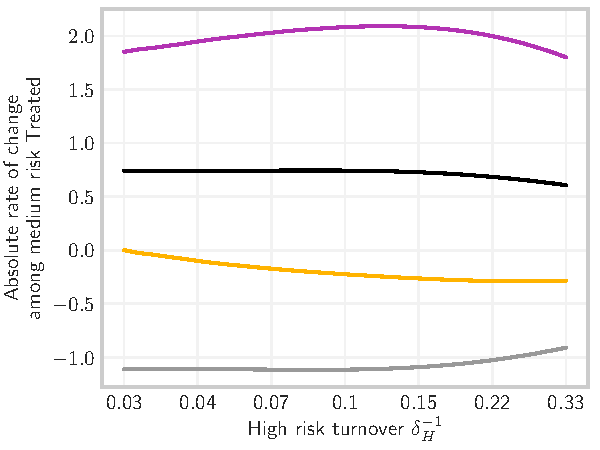
\includegraphics[width=\linewidth]{dX-abs-full-med-T.pdf}
    \caption{Medium risk treated}\label{fig:dX-app-med-T}
  \end{subfigure}\\
  \begin{subfigure}{0.33\linewidth}
    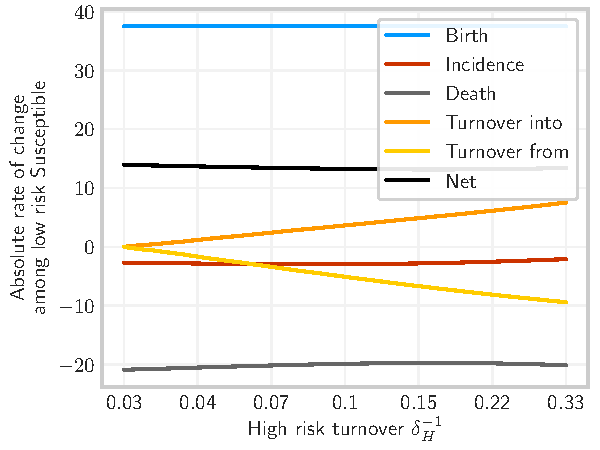
\includegraphics[width=\linewidth]{dX-abs-full-low-S.pdf}
    \caption{Low risk susceptible}\label{fig:dX-app-low-S}
  \end{subfigure}%
  \begin{subfigure}{0.33\linewidth}
    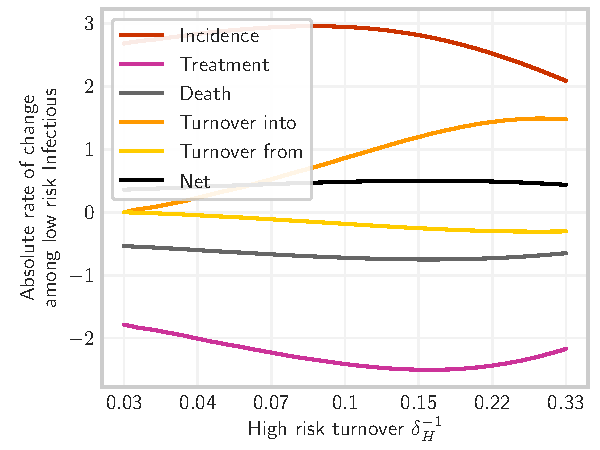
\includegraphics[width=\linewidth]{dX-abs-full-low-I.pdf}
    \caption{Low risk infectious}\label{fig:dX-app-low-I}
  \end{subfigure}%
  \begin{subfigure}{0.33\linewidth}
    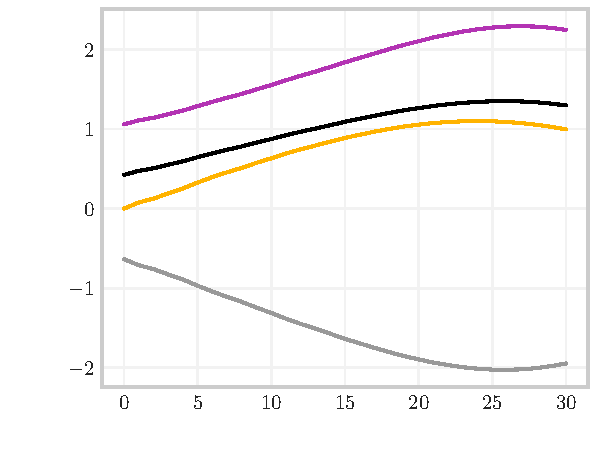
\includegraphics[width=\linewidth]{dX-abs-full-low-T.pdf}
    \caption{Low risk treated}\label{fig:dX-app-low-T}
  \end{subfigure}\\
  \endgroup
  \caption{Absolute rates of change at equilibrium
    (number of individuals gained/lost per year)
    among individuals in each health state and risk group,
    broken down by type of change:
    gain via births,
    loss/gain via incident infections,
    loss/gain via treatment,
    loss/gain via turnover,
    loss via death,
    and net change.
    Based on Eq.~(\ref{eq:model}).}
  \label{fig:dX-app}
  \footnotesizeTurnover rate (log scale) is a function of
the duration of time spent in the high risk group $\delta_H$,
where shorter time spent in the high risk group yields faster turnover.
No turnover is indicated by $\delta_H^{-1} = 0.03$,
due to population exit rate $\mu = 0.03$.
  Rates of change do not sum to zero due to population growth.
\end{figure}
\begin{figure}[H]
  \centerline{\includegraphics[width=0.5\linewidth]{{2d-tip-all-tau=0.1}.pdf}}
  \caption{Proportion of new infectious individuals in each risk group
    which are from turnover of infectious individuals,
    as opposed to incident infection of susceptible individuals in the risk group.}
  \label{fig:new-inf-phi-vs-lambda}
\end{figure}
% ==================================================================================================
\subsection{Equilibrium Prevalence Ratios}
\begin{figure}[H]
  \begingroup\centering
  \begin{subfigure}{0.33\linewidth}
    \includegraphics[width=\linewidth]{{1d-ratio-prevalence-high-low-tau=0.1}.pdf}
    \caption{High vs Low risk}
    \label{fig:1d-ratio-prevalence-high-low}
  \end{subfigure}%
  \begin{subfigure}{0.33\linewidth}
    \includegraphics[width=\linewidth]{{1d-ratio-prevalence-high-med-tau=0.1}.pdf}
    \caption{High vs Medium Risk}
    \label{fig:1d-ratio-prevalence-high-med}
  \end{subfigure}%
  \begin{subfigure}{0.33\linewidth}
    \includegraphics[width=\linewidth]{{1d-ratio-prevalence-med-low-tau=0.1}.pdf}
    \caption{Medium vs Low Risk}
    \label{fig:1d-ratio-prevalence-med-low}
  \end{subfigure}%
  \\\endgroup
  \caption{Equilibrium prevalence ratios between risk groups
    under different rates of turnover.}
  \label{fig:1d-ratio-prevalence}
  \footnotesizeTurnover rate (log scale) is a function of
the duration of time spent in the high risk group $\delta_H$,
where shorter time spent in the high risk group yields faster turnover.
No turnover is indicated by $\delta_H^{-1} = 0.03$,
due to population exit rate $\mu = 0.03$.
\end{figure}
% ==================================================================================================
\subsection{Equilibrium Incidence}
\begin{figure}[H]
  \begingroup\centering
  \begin{subfigure}{0.33\linewidth}
    \includegraphics[width=\linewidth]{{1d-incidence-high-tau=0.1}.pdf}
    \caption{High risk}
    \label{fig:1d-incidence-high}
  \end{subfigure}%
  \begin{subfigure}{0.33\linewidth}
    \includegraphics[width=\linewidth]{{1d-incidence-med-tau=0.1}.pdf}
    \caption{Medium risk}
    \label{fig:1d-incidence-med}
  \end{subfigure}%
  \begin{subfigure}{0.33\linewidth}
    \includegraphics[width=\linewidth]{{1d-incidence-low-tau=0.1}.pdf}
    \caption{Low risk}
    \label{fig:1d-incidence-low}
  \end{subfigure}%
  \\\endgroup
  \caption{Equilibrium incidence among high, medium, and low risk groups
    under different rates of turnover.}
  \label{fig:1d-incidence}
  \footnotesizeTurnover rate (log scale) is a function of
the duration of time spent in the high risk group $\delta_H$,
where shorter time spent in the high risk group yields faster turnover.
No turnover is indicated by $\delta_H^{-1} = 0.03$,
due to population exit rate $\mu = 0.03$.
  Incidence in each risk group is proportional to overall incidence
  with $C_i$ as a scale factor.
\end{figure}
\begin{figure}[H]
  \begingroup\centering
  \begin{subfigure}{0.33\linewidth}
    \includegraphics[width=\linewidth]{{1d-ratio-incidence-high-low-tau=0.1}.pdf}
    \caption{High vs low risk}
    \label{fig:1d-ratio-incidence-high-low}
  \end{subfigure}%
  \begin{subfigure}{0.33\linewidth}
    \includegraphics[width=\linewidth]{{1d-ratio-incidence-high-med-tau=0.1}.pdf}
    \caption{High vs medium risk}
    \label{fig:1d-ratio-incidence-high-med}
  \end{subfigure}%
  \begin{subfigure}{0.33\linewidth}
    \includegraphics[width=\linewidth]{{1d-ratio-incidence-med-low-tau=0.1}.pdf}
    \caption{Medium vs low risk}
    \label{fig:1d-ratio-incidence-med-low}
  \end{subfigure}
  \\\endgroup
  \caption{Equilibrium incidence ratios between risk groups
    under different rates of turnover.
    Incidence ratios do not depend on turnover.}
  \label{fig:1d-ratio-incidence}
  \footnotesizeTurnover rate (log scale) is a function of
the duration of time spent in the high risk group $\delta_H$,
where shorter time spent in the high risk group yields faster turnover.
No turnover is indicated by $\delta_H^{-1} = 0.03$,
due to population exit rate $\mu = 0.03$.
\end{figure}
% ==================================================================================================
\subsection{Equilibrium prevalence and number of partners before and after model fitting}
\begin{figure}[H]
  \begingroup\centering
  \begin{subfigure}{0.4\linewidth}
    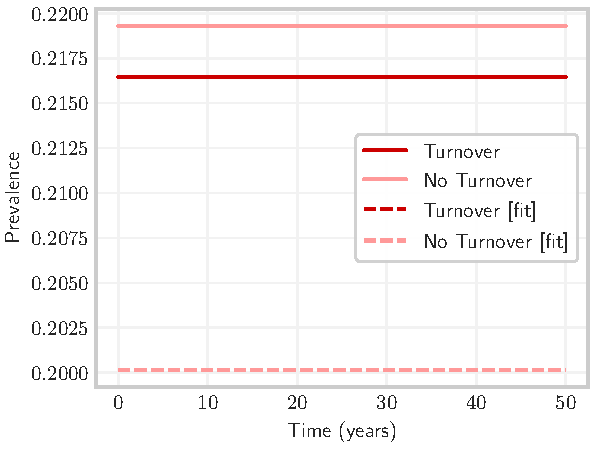
\includegraphics[width=\linewidth]{main-tpaf-prevalence-high}
    \caption{High risk}
    \label{fig:tpaf-prevalence-high}
  \end{subfigure}
  \begin{subfigure}{0.4\linewidth}
    \centering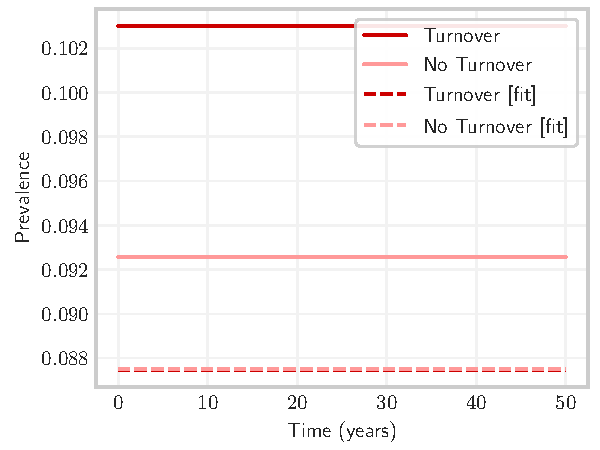
\includegraphics[width=\linewidth]{main-tpaf-prevalence-med}
    \caption{Medium risk}
    \label{fig:tpaf-prevalence-med}
  \end{subfigure}
  \begin{subfigure}{0.4\linewidth}
    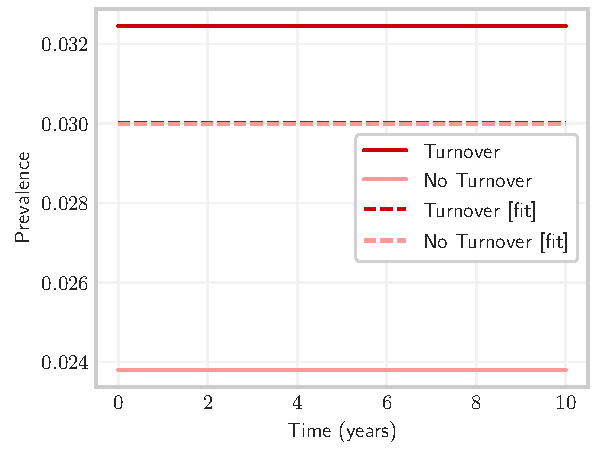
\includegraphics[width=\linewidth]{main-tpaf-prevalence-low}
    \caption{Low risk}
    \label{fig:tpaf-prevalence-low}
  \end{subfigure}
  \begin{subfigure}{0.4\linewidth}
    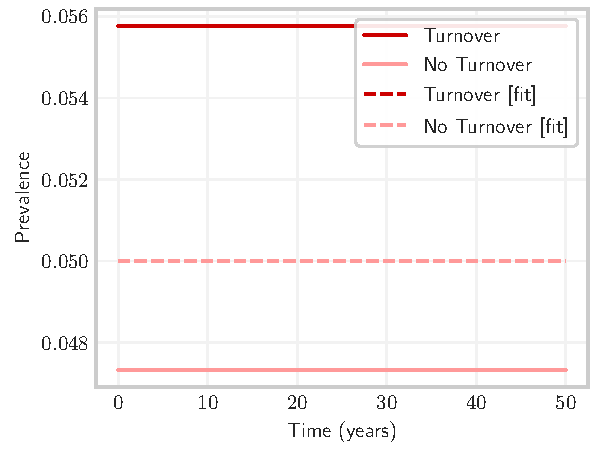
\includegraphics[width=\linewidth]{main-tpaf-prevalence-all}
    \caption{Overall}
    \label{fig:tpaf-prevalence-all}
  \end{subfigure}
  \\\endgroup
  \caption{Equilibrium STI prevalence
    among high, medium, and low risk groups as well as overall,
    with and without turnover,
    and with and without fitted $C_i$ to group-specific prevalence.}
  \label{fig:tpaf-prevalence}
\end{figure}
\begin{figure}[H]
  \begingroup\centering
  \begin{subfigure}{0.4\linewidth}
    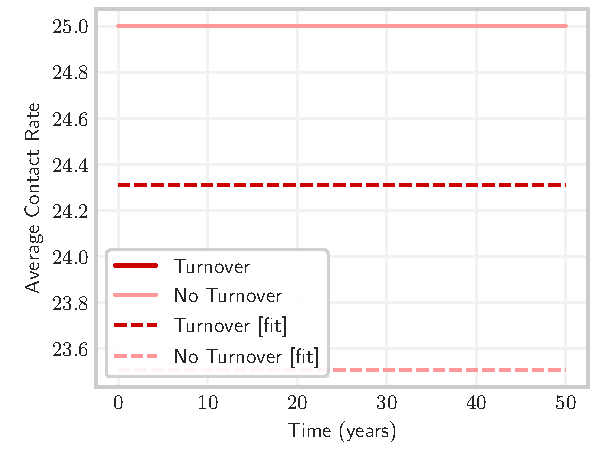
\includegraphics[width=\linewidth]{main-tpaf-C-high}
    \caption{High risk}
    \label{fig:tpaf-C-high}
  \end{subfigure}
  \begin{subfigure}{0.4\linewidth}
    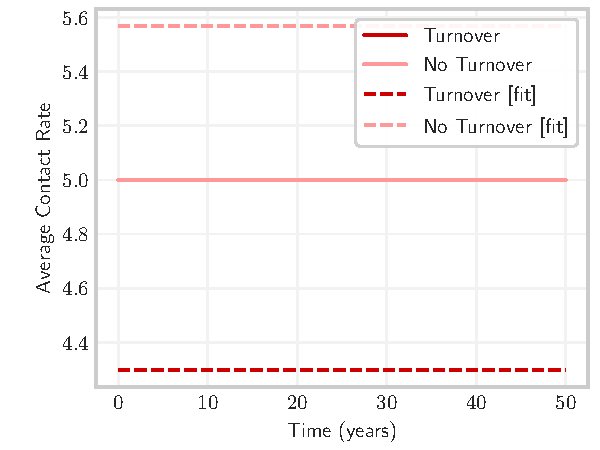
\includegraphics[width=\linewidth]{main-tpaf-C-med}
    \caption{Medium risk}
    \label{fig:tpaf-C-med}
  \end{subfigure}
  \begin{subfigure}{0.4\linewidth}
    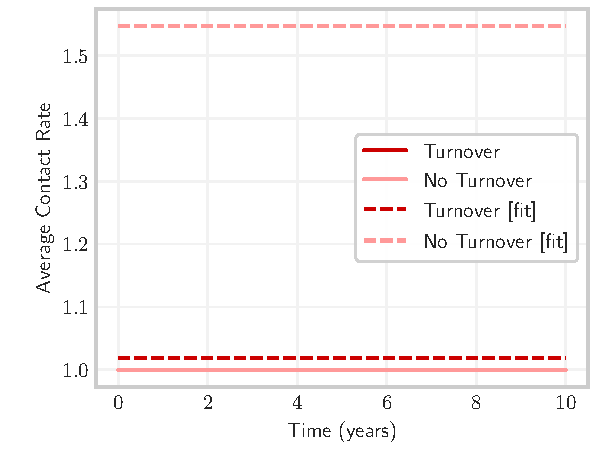
\includegraphics[width=\linewidth]{main-tpaf-C-low}
    \caption{Low risk}
    \label{fig:tpaf-C-low}
  \end{subfigure}
  \begin{subfigure}{0.4\linewidth}
    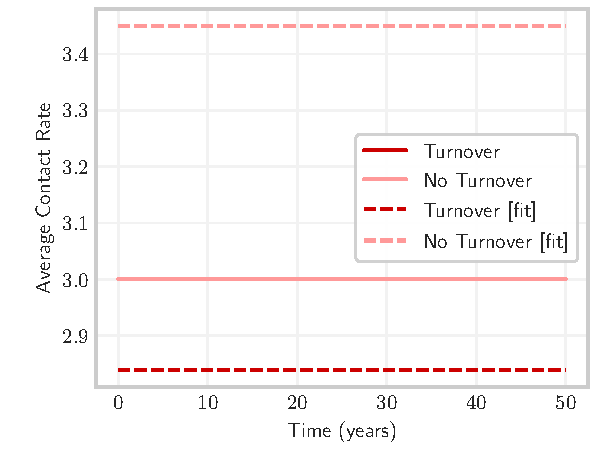
\includegraphics[width=\linewidth]{main-tpaf-C-all}
    \caption{Overall}
    \label{fig:tpaf-C-all}
  \end{subfigure}
  \\\endgroup
  \caption{Numbers of partners $C_i$
    among high, medium, and low risk groups as well as overall,
    with and without turnover,
    and with and without model fitting to group-specific prevalence.}
  \label{fig:tpaf-C}
\end{figure}
% ==================================================================================================
\subsection{Influence of turnover on tPAF of the high and medium risk groups before and after model fitting}
\begin{figure}[H]
  \begingroup\centering
  \begin{subfigure}{0.4\linewidth}
    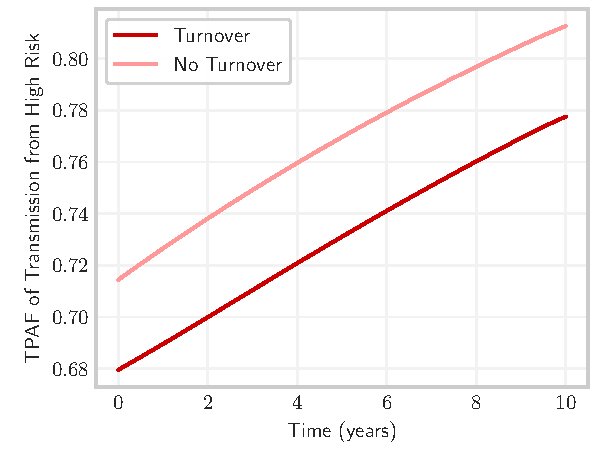
\includegraphics[width=\linewidth]{main-tpaf-tpaf-high-all-vs=raw}
    \caption{High risk, before fitting}
    \label{fig:tpaf-high-raw}
  \end{subfigure}
  \begin{subfigure}{0.4\linewidth}
    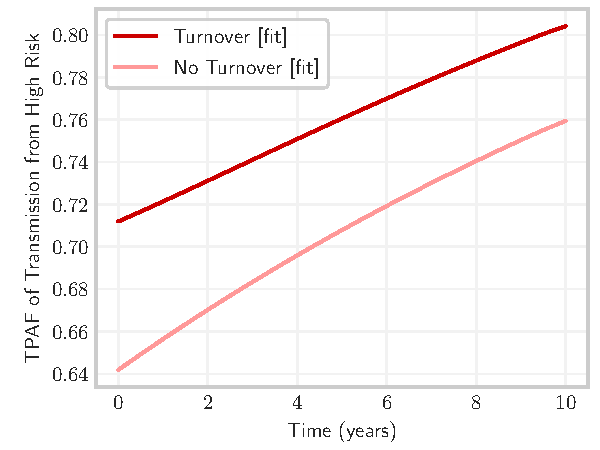
\includegraphics[width=\linewidth]{main-tpaf-tpaf-high-all-vs=fit}
    \caption{High risk, after fitting}
    \label{fig:tpaf-high-fit}
  \end{subfigure}
  \begin{subfigure}{0.4\linewidth}
    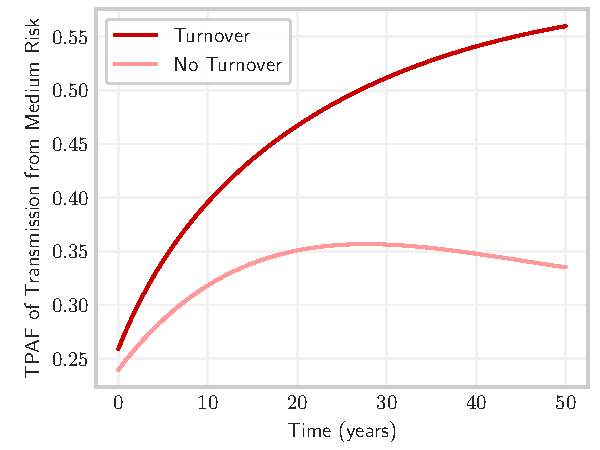
\includegraphics[width=\linewidth]{main-tpaf-tpaf-med-all-vs=raw}
    \caption{Medium risk, before fitting}
    \label{fig:tpaf-med-raw}
  \end{subfigure}
  \begin{subfigure}{0.4\linewidth}
    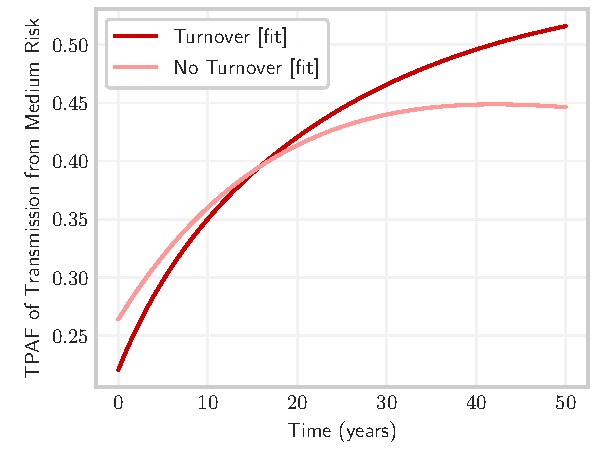
\includegraphics[width=\linewidth]{main-tpaf-tpaf-med-all-vs=fit}
    \caption{Medium risk, after fitting}
    \label{fig:tpaf-med-fit}
  \end{subfigure}
  \\\endgroup
  \caption{Transmission population attributable fraction (tPAF)
    of the high and medium risk groups in models with and without turnover,
    before and after model fitting.}
\end{figure}
% ==================================================================================================
\subsection{Effect of treatment rate on the influence of turnover on equilibrium prevalence}
In order to examine the effect of treatment rate $\tau$ on
the results of Experiment~1
-- the influence of turnover on equilibrium prevalence --
we recreated Figures~\ref{fig:prevalence}~and~\ref{fig:incidence-factors}
for a range of treatment rates $\tau \in [0.05, 1.0]$.
The results are shown in Figure~\ref{fig:2d}.
\begin{figure}[H]
  \begin{minipage}{0.5\linewidth}
    \begingroup\centering
    \begin{subfigure}{0.8\linewidth}
      \includegraphics[width=\linewidth]{{2d-prevalence-high}.pdf}
      \caption{Prevalence among high risk}
      \label{fig:2d-prevalence-high}
    \end{subfigure}\\
    \begin{subfigure}{0.8\linewidth}
      \includegraphics[width=\linewidth]{{2d-prevalence-med}.pdf}
      \caption{Prevalence among medium risk}
      \label{fig:2d-prevalence-med}
    \end{subfigure}\\
    \begin{subfigure}{0.8\linewidth}
      \includegraphics[width=\linewidth]{{2d-prevalence-low}.pdf}
      \caption{Prevalence among low risk}
      \label{fig:2d-prevalence-low}
    \end{subfigure}\\
    \endgroup
  \end{minipage}%
  \begin{minipage}{0.5\linewidth}
    \begingroup\centering
    \begin{subfigure}[t]{0.8\linewidth}
      \includegraphics[width=\linewidth]{{2d-C-I}.pdf}
      \caption{Average $C$ among infectious individuals $\hat{C}_{\mathcal{I}}$}
      \label{fig:2d-C-I}
    \end{subfigure}\\
    \begin{subfigure}[t]{0.8\linewidth}
      \includegraphics[width=\linewidth]{{2d-prevalence-all}.pdf}
      \caption{Prevalence overall}
      \label{fig:2d-prev-all}
    \end{subfigure}\\
    \begin{subfigure}[t]{0.8\linewidth}
      \includegraphics[width=\linewidth]{{2d-incidence-all}.pdf}
      \caption{Incidence overall $\lambda$}
      \label{fig:2d-incidence-all}
    \end{subfigure}\\
    \endgroup
  \end{minipage}
  \caption{Relationship between turnover rate and
    equilibrium STI prevalence in high, medium, and low risk groups,
    as well as overall STI prevalence and incidence,
    and average $C$ among infectious individuals,
    for a range of treatment rates $\tau$.
    Darker blue indicates higher treatment rate.
    The threshold turnover rate separating regions~A~and~B
    decreases with treatment rate, meaning that
    increasing turnover becomes more likely to decrease equilibrium prevalence
    as treatment rate increases.}
  \label{fig:2d}
  \footnotesizeTurnover rate (log scale) is a function of
the duration of time spent in the high risk group $\delta_H$,
where shorter time spent in the high risk group yields faster turnover.
No turnover is indicated by $\delta_H^{-1} = 0.03$,
due to population exit rate $\mu = 0.03$.
\end{figure}